\section{النشر والاعتماد}
\label{sec:settings-feature-publishing-approval}

تحدد هذه الصفحة التغييرات التي يجب أن يراجعها شخص آخر قبل أن تصل إلى الأعضاء، فلا يتأثر العمل اليومي بتعديل متسرع. ولها ثلاثة تبويبات مستقلة، ولكل منها سياسته وزر حفظه: «النماذج» و«أنواع السجلات» و«بطاقات الإجراءات». وتبقى السياسة متوقفة حتى تشغّلها. تظهر الصفحة لمالك المؤسسة ولمن يحمل دور المسؤول، ويختلف ما يراه غيرهم بحسب التبويب.

\begin{rcnote}[مثال: شركة الأفق]
يختار مسؤول النظام «لكل النماذج» عند ①، ويكتب مرحلة باسم «مراجعة الموارد البشرية» عند ②، ويعيّن سارة الخطيب مراجعة، ثم يضغط «حفظ» عند ⑤. فإذا عدّل عمر حداد نموذج طلب الزيارة، لا يُنشر الإصدار الجديد قبل أن تعتمده سارة.
\end{rcnote}

\begin{figure}[H]
\centering
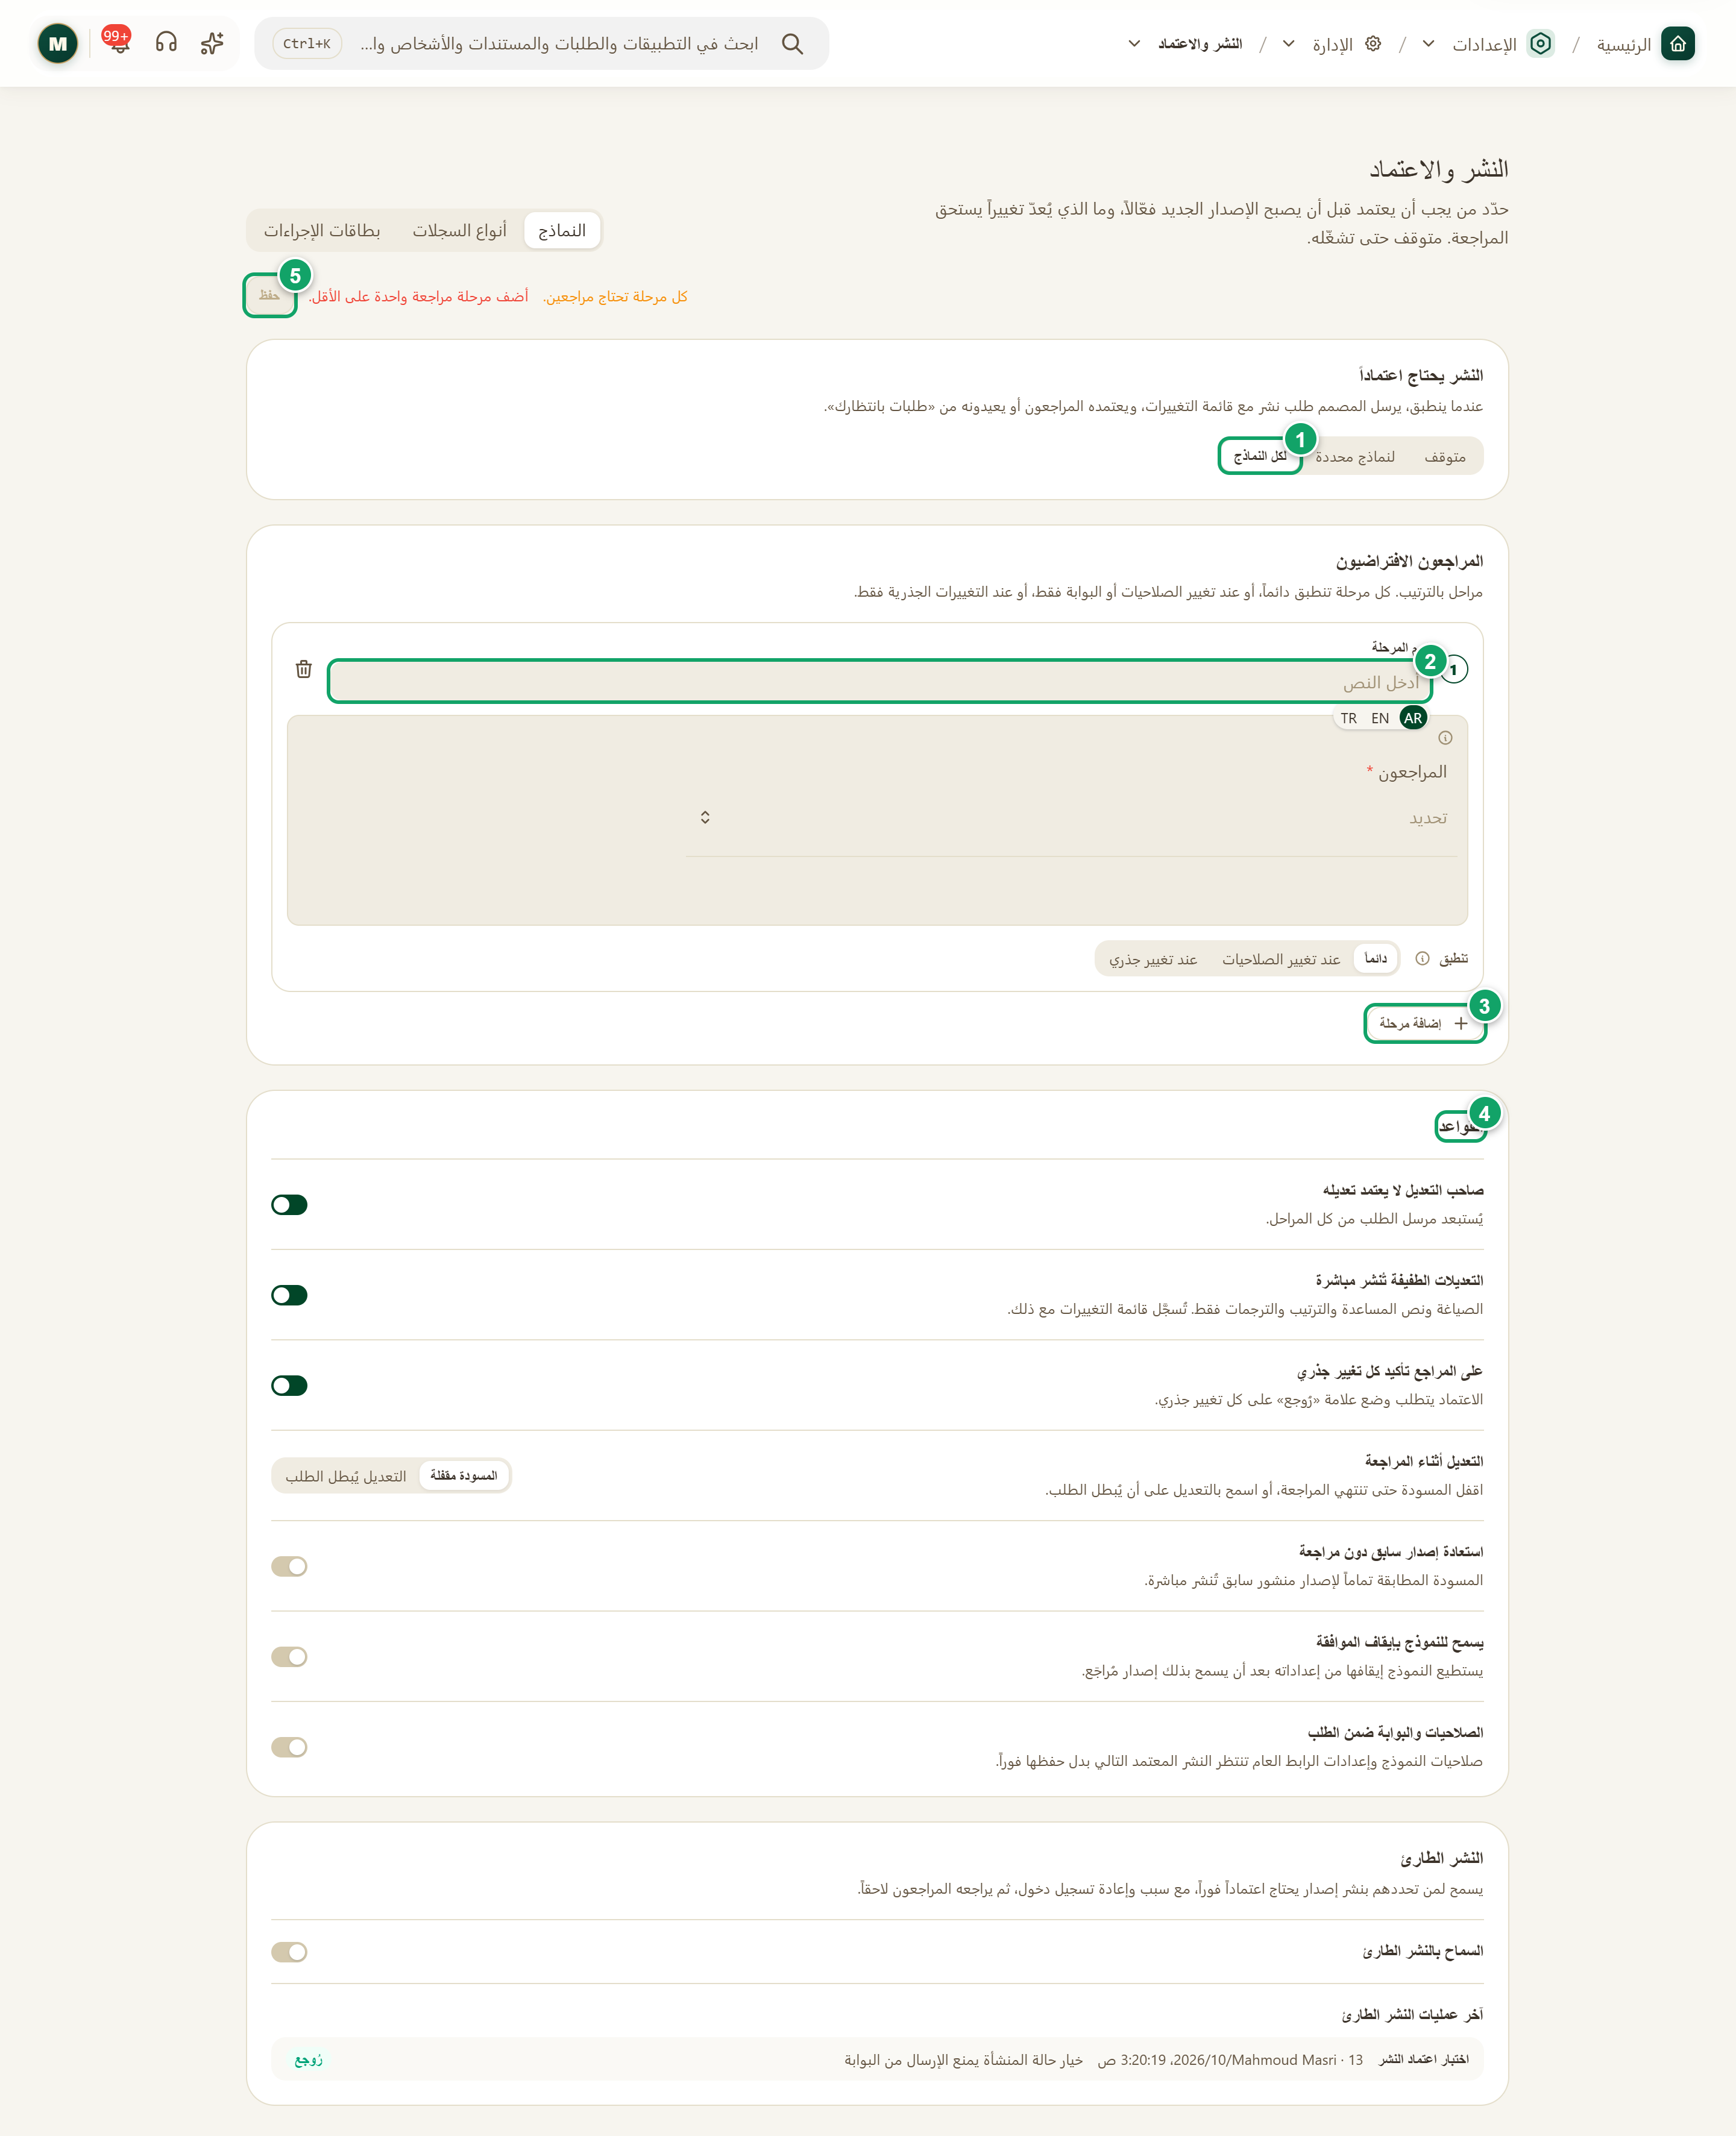
\includegraphics[width=0.95\linewidth,height=0.72\textheight,keepaspectratio]{figures/screens/ch08-publishing-approval-ar.png}
\caption{سياسة النشر في تبويب النماذج}
\label{fig:settings-publishing-approval-screen}
\shotnote{تعرض الصورة تعديلاً تجريبياً لم يُحفظ: اختير «لكل النماذج» وأُضيفت مرحلة فارغة، فظهر تنبيهان وبقي الحفظ معطلاً. فالسياسة لا تُحفظ قبل أن تحدد من يراجع. وتعرض «آخر عمليات النشر الطارئ» سجلاً من بيانات الاختبار. ① «لكل النماذج»: نطاق السياسة. ② «اسم المرحلة». ③ «إضافة مرحلة». ④ «القواعد». ⑤ «حفظ».}
\end{figure}

\begin{table}[H]
\centering
\caption{ماذا تسجل في تبويب النماذج؟}
\label{tab:settings-publishing-approval-forms}
\begin{tabularx}{\linewidth}{R{4.2cm} Y}
\rcHeaderRow
\thh{الإعداد} & \thh{ما الذي تحدده؟}\\
«النشر يحتاج اعتماداً» & «متوقف» أو «لنماذج محددة» أو «لكل النماذج».\\
«النماذج المشمولة» & يظهر مع «لنماذج محددة»: «المتاحة على البوابة أو عبر خدمة» و«التي فيها خطوات موافقة» و«التي تكتب في السجلات».\\
«المراجعون الافتراضيون» & مراحل متتابعة، حتى 6 مراحل. لكل مرحلة «اسم المرحلة» و«المراجعون» و«تنطبق»: «دائماً» أو «عند تغيير الصلاحيات» أو «عند تغيير جذري».\\
«صاحب التعديل لا يعتمد تعديله» & يُستبعد مرسل الطلب من كل المراحل.\\
«التعديلات الطفيفة تُنشر مباشرة» & الصياغة ونص المساعدة والترتيب والترجمات لا تحتاج إلى مراجعة، وتبقى مسجلة في قائمة التغييرات.\\
«على المراجع تأكيد كل تغيير جذري» & التغيير الجذري هو حذف سؤال أو خيار أو تغيير نوع سؤال أو طريقة كتابة الإجابات في السجلات. ويلزم المراجع وضع علامة «رُوجع» على كل واحد منها.\\
«التعديل أثناء المراجعة» & «المسودة مقفلة» حتى تنتهي المراجعة، أو «التعديل يُبطل الطلب».\\
«استعادة إصدار سابق دون مراجعة» & المسودة المطابقة تماماً لإصدار منشور سابق تُنشر مباشرة.\\
«يسمح للنموذج بإيقاف الموافقة» & يستطيع النموذج إيقافها من إعداداته بعد أن يسمح بذلك إصدار مُراجَع.\\
«الصلاحيات والبوابة ضمن الطلب» & تنتظر صلاحيات النموذج وإعدادات رابطه العام النشر المعتمد التالي بدل حفظها فوراً.\\
«النشر الطارئ» & عند تفعيله تحدد «من يحق له النشر الطارئ» و«المراجعة اللاحقة خلال» من يوم إلى 14 يوماً. ينشر هؤلاء فوراً بعد كتابة سبب وإعادة تسجيل الدخول، ثم يراجع المراجعون الإصدار لاحقاً.\\
\end{tabularx}
\end{table}

\begin{figure}[H]
\centering
\begin{tikzpicture}[node distance=0.5cm]
\node[stepBox] (a) {\RL{يكتب المصمم المسودة}};
\node[stepBox,below=of a] (b) {\RL{يرسل طلب نشر مع قائمة التغييرات}};
\node[stepBox,below=of b] (c) {\RL{يراجعه المراجعون مرحلة بعد مرحلة}};
\node[stepBox,below=of c] (d) {\RL{يصبح الإصدار فعّالاً بعد الاعتماد}};
\draw[flowsTo] (a) -- (b);
\draw[flowsTo] (b) -- (c);
\draw[flowsTo] (c) -- (d);
\end{tikzpicture}
\rclegend
\caption{طريق إصدار النموذج عند تشغيل السياسة}
\label{fig:settings-publishing-approval-flow}
\shotnote{يوضح المخطط ما يتغير على مصممي النماذج بعد تشغيل السياسة: يصبح النشر طلباً يصل إلى المراجعين في «طلبات بانتظارك»، فيعتمدونه أو يعيدونه. ويبقى الإصدار الحالي في العمل طوال هذه المدة، لذلك أبلغ المصممين قبل التشغيل.}
\end{figure}

\begin{figure}[H]
\centering
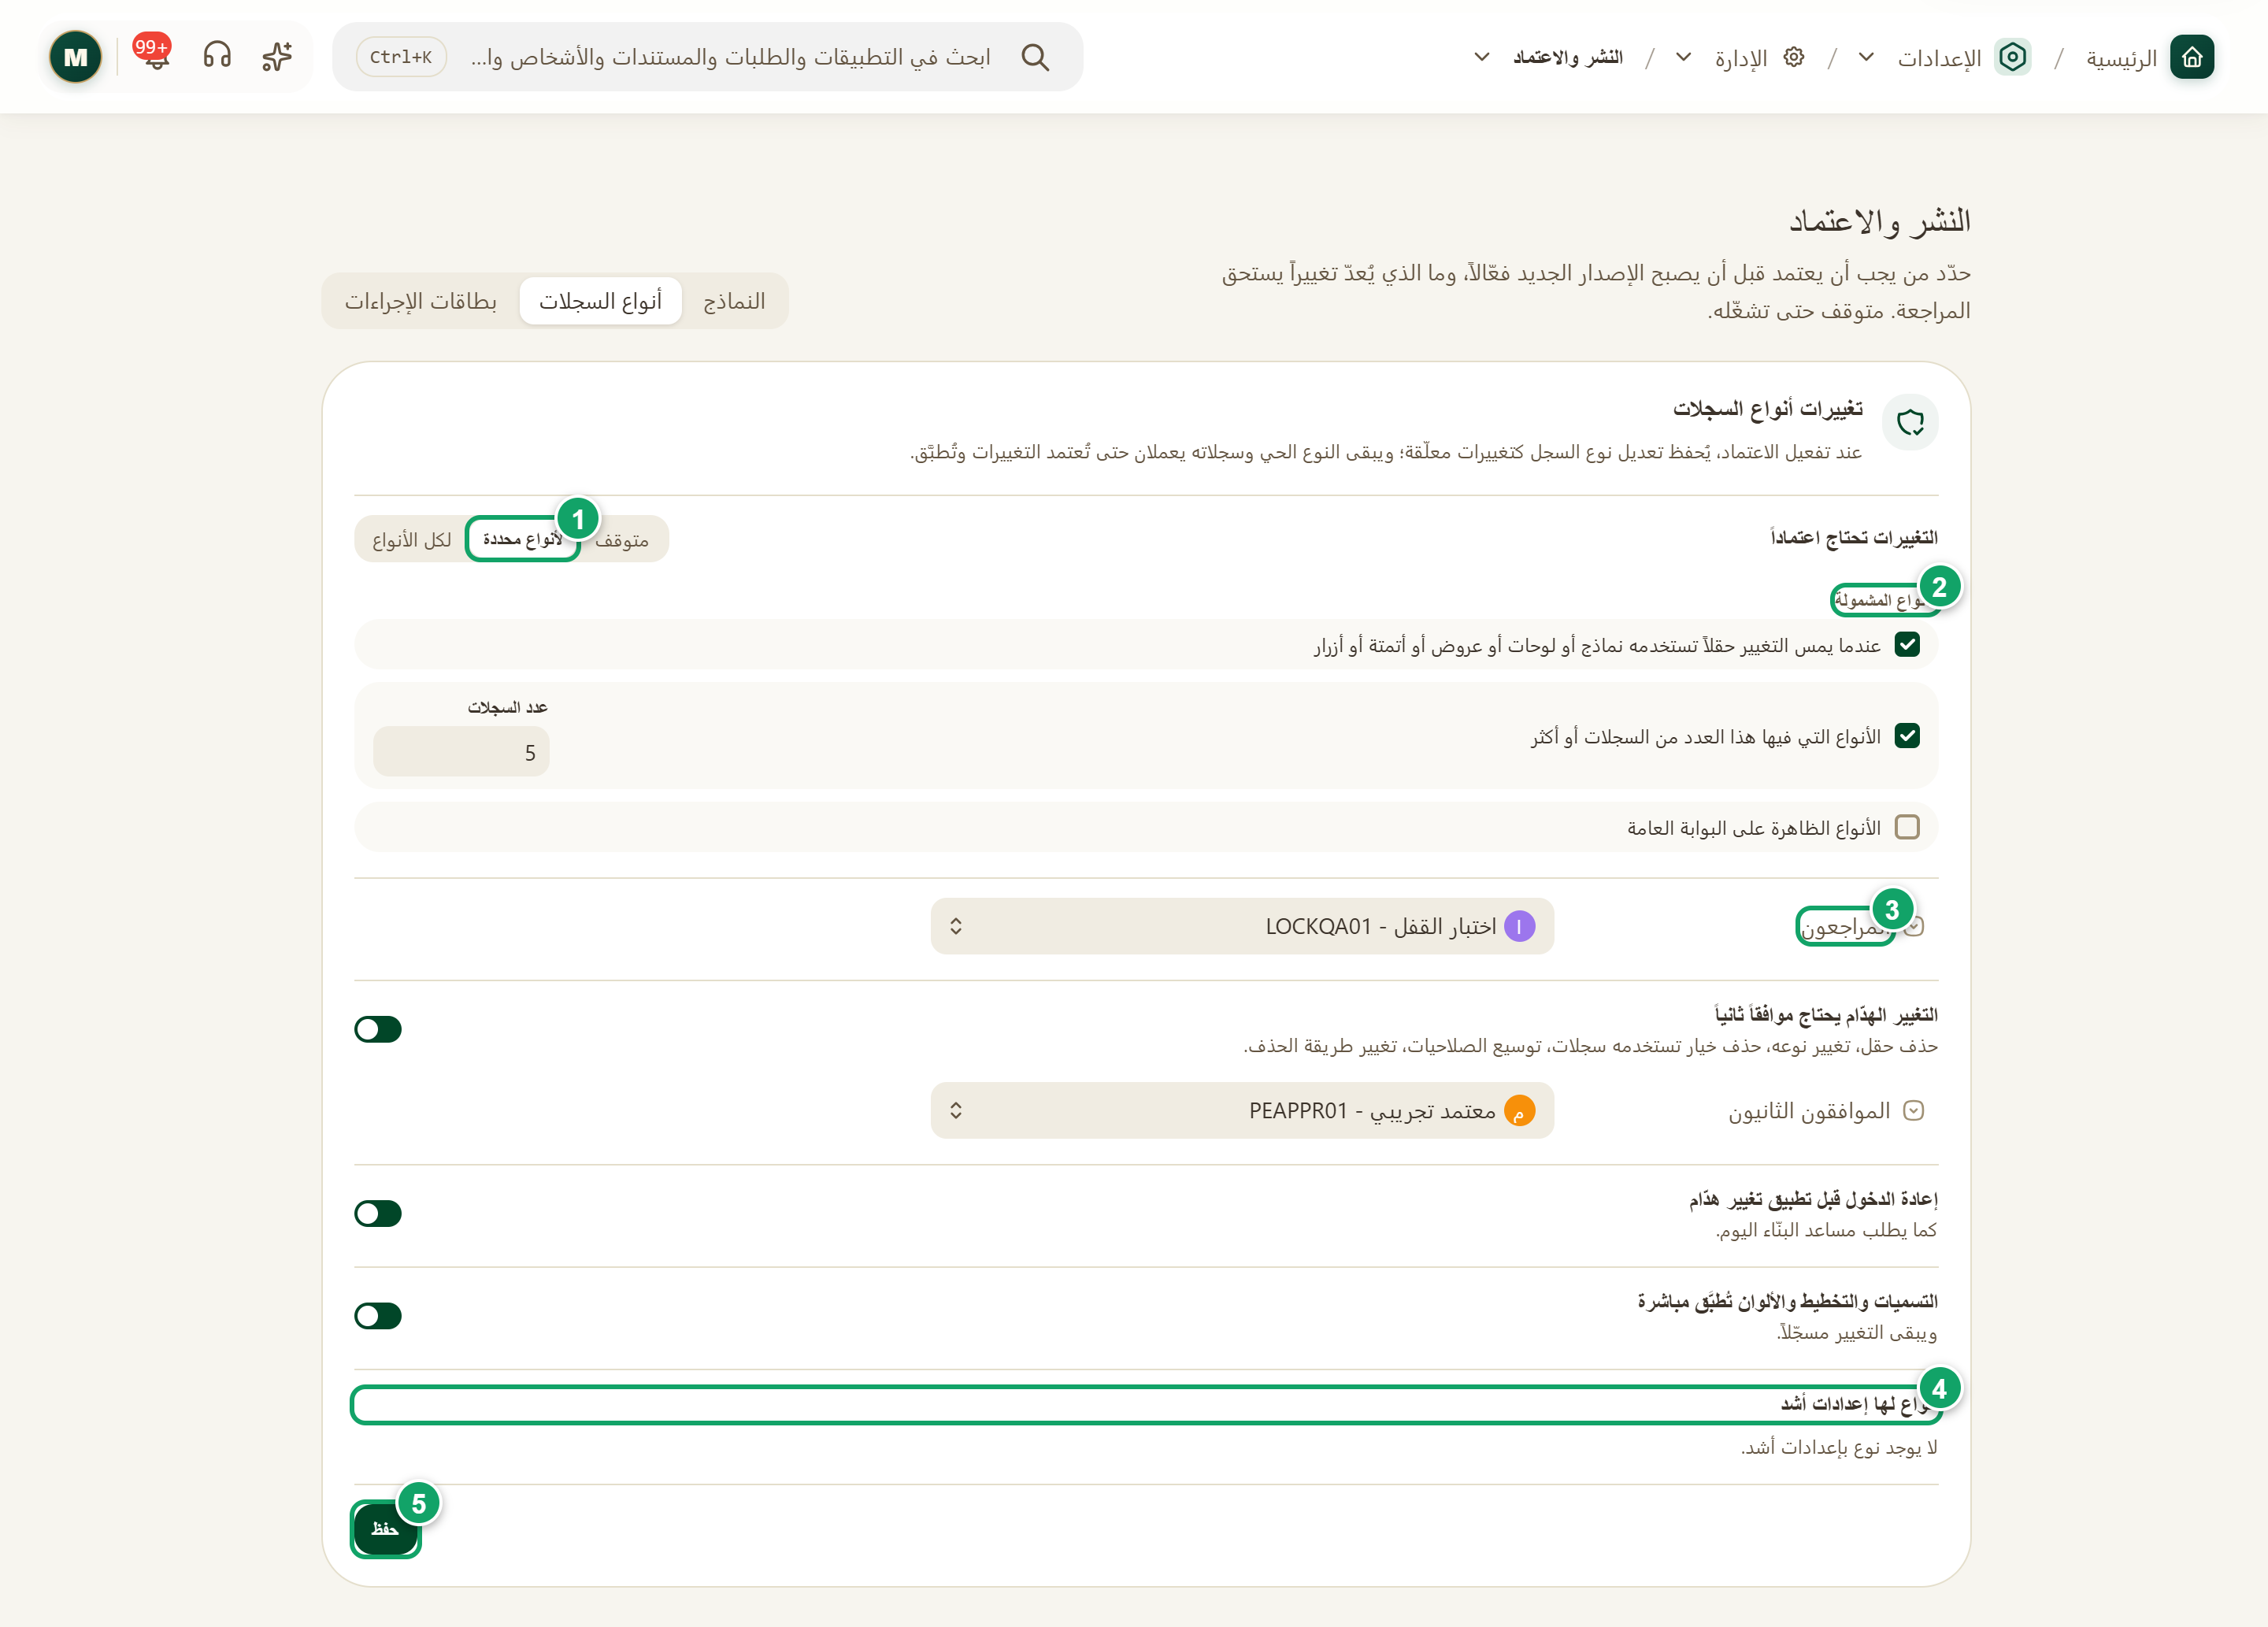
\includegraphics[width=0.95\linewidth,height=0.72\textheight,keepaspectratio]{figures/screens/ch08-publishing-approval-record-types-ar.png}
\caption{سياسة تبويب أنواع السجلات}
\label{fig:settings-publishing-approval-record-types-screen}
\shotnote{تعرض الصورة اختيار «لأنواع محددة» دون حفظ، وهو اختيار يكشف الحقول المخفية، أما السياسة المحفوظة في مؤسسة الاختبار فمتوقفة. وعند التشغيل يبقى النوع الحالي وسجلاته يعملان حتى تُعتمد التغييرات المعلّقة وتُطبَّق. ① «لأنواع محددة». ② «الأنواع المشمولة». ③ «المراجعون»: يكفي اعتماد أحدهم، ولا يُحتسب اعتماد من أجرى التغييرات. ④ «أنواع لها إعدادات أشد». ⑤ «حفظ».}
\end{figure}

\begin{table}[H]
\centering
\caption{ماذا تسجل في تبويب أنواع السجلات؟}
\label{tab:settings-publishing-approval-record-types}
\begin{tabularx}{\linewidth}{R{4.2cm} Y}
\rcHeaderRow
\thh{الإعداد} & \thh{ما الذي تحدده؟}\\
«التغييرات تحتاج اعتماداً» & «متوقف» أو «لأنواع محددة» أو «لكل الأنواع».\\
«الأنواع المشمولة» & تغيير يمس حقلاً تستخدمه نماذج أو لوحات أو عروض أو أتمتة أو أزرار، أو الأنواع التي بلغت «عدد السجلات» المحدد، أو الأنواع الظاهرة على البوابة العامة.\\
«التغيير الهدّام يحتاج موافقاً ثانياً» & حذف حقل، أو تغيير نوعه، أو حذف خيار تستخدمه سجلات، أو توسيع الصلاحيات، أو تغيير طريقة الحذف. وتحدد معه «الموافقون الثانيون».\\
«إعادة الدخول قبل تطبيق تغيير هدّام» & يعيد الشخص تسجيل دخوله قبل التطبيق.\\
«التسميات والتخطيط والألوان تُطبَّق مباشرة» & لا تنتظر هذه التغييرات الاعتماد، ويبقى التغيير مسجلاً.\\
«أنواع لها إعدادات أشد» & قائمة الأنواع التي لها قواعد خاصة أشد من السياسة العامة، ويزيل زر «إزالة» القاعدة الخاصة.\\
\end{tabularx}
\end{table}

\begin{figure}[H]
\centering
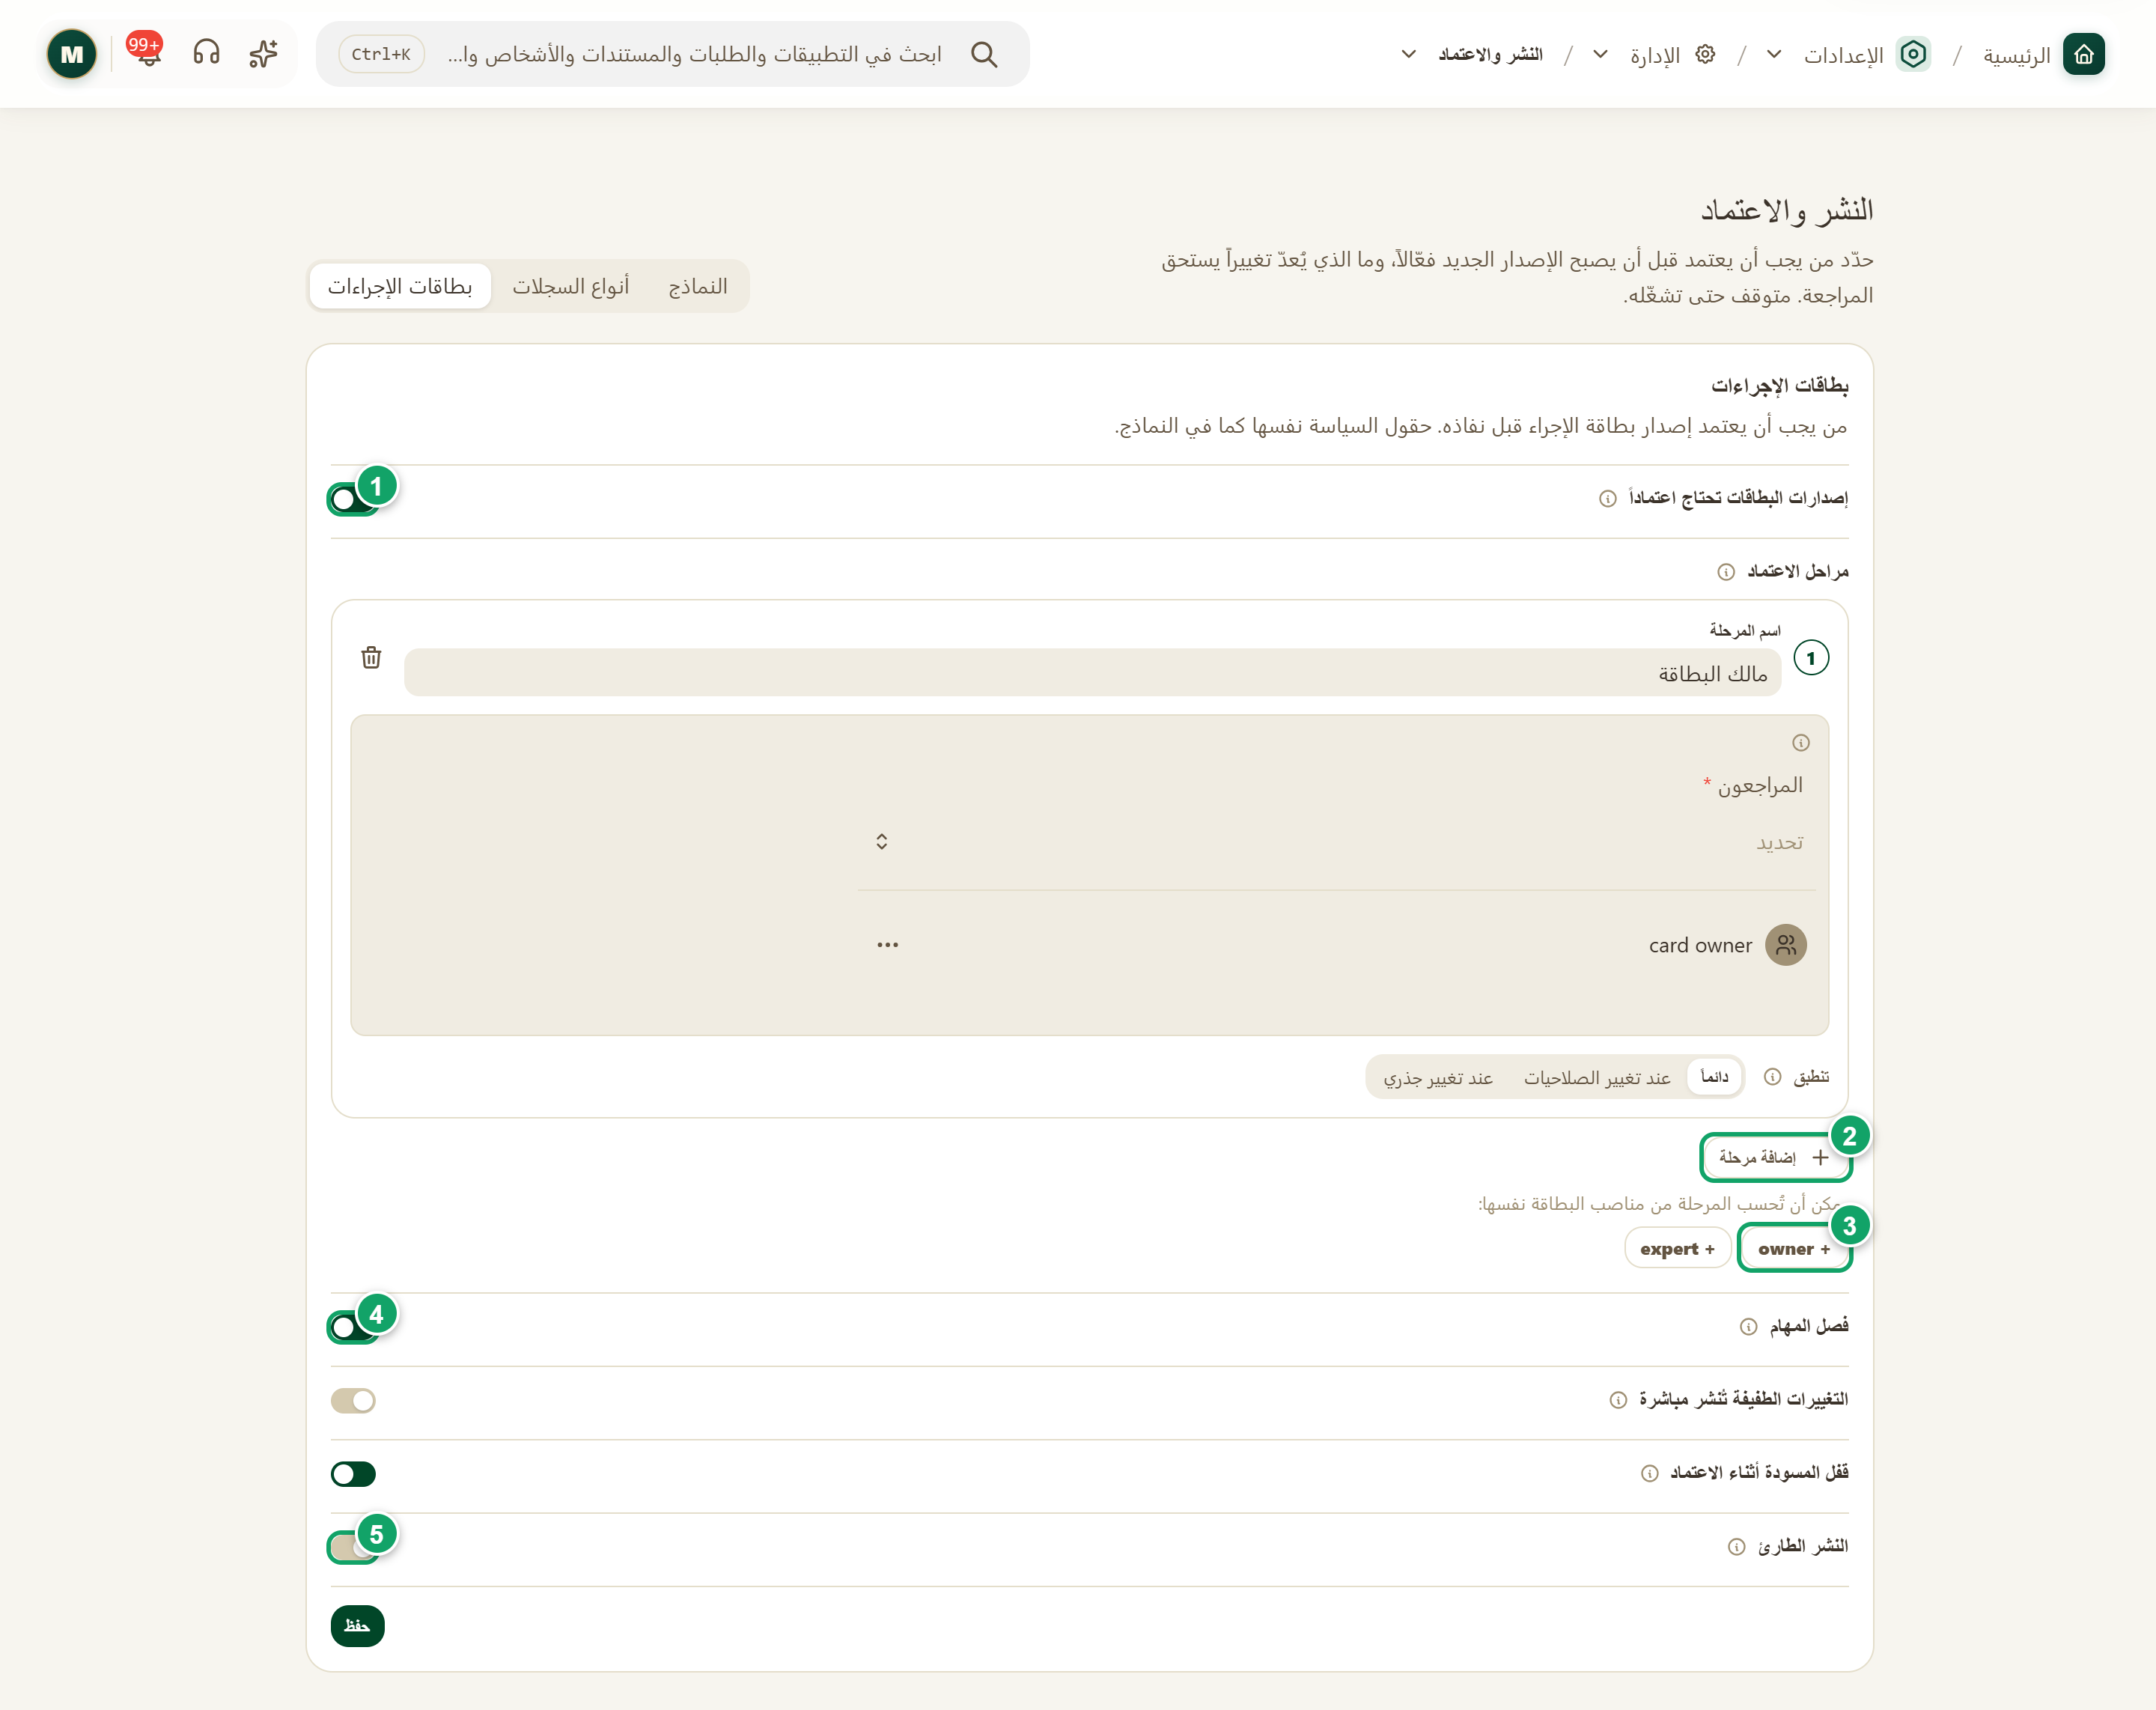
\includegraphics[width=0.95\linewidth,height=0.72\textheight,keepaspectratio]{figures/screens/ch08-publishing-approval-procedure-cards-ar.png}
\caption{سياسة تبويب بطاقات الإجراءات}
\label{fig:settings-publishing-approval-procedure-cards-screen}
\shotnote{تعرض الصورة سياسة مفعلة في مؤسسة الاختبار، ومرحلتها الوحيدة يتولاها مالك البطاقة. فهذا التبويب يمنع العمل بإصدار بطاقة إجراء قبل اعتماده، وقد ظهرت أسماء المناصب فيه بالإنجليزية في النسختين. ① «إصدارات البطاقات تحتاج اعتماداً». ② «إضافة مرحلة». ③ الزر \en{+ owner}: يضيف مرحلة يتولاها مالك البطاقة، ويقابله \en{+ expert} لخبير البطاقة. ④ «فصل المهام»: محرر المسودة لا يعتمد مسودته. ⑤ «النشر الطارئ».}
\end{figure}

\begin{table}[H]
\centering
\caption{ماذا تسجل في تبويب بطاقات الإجراءات؟}
\label{tab:settings-publishing-approval-procedure-cards}
\begin{tabularx}{\linewidth}{R{4.2cm} Y}
\rcHeaderRow
\thh{الإعداد} & \thh{ما الذي تحدده؟}\\
«مراحل الاعتماد» & من يعتمد وبأي ترتيب، ومتى تنطبق كل مرحلة. ويمكن أن تُحسب المرحلة من مناصب البطاقة نفسها.\\
«التغييرات الطفيفة تُنشر مباشرة» & حين تكون كل التغييرات طفيفة، مثل الصياغة والترتيب، يُنشر الإصدار دون اعتماد.\\
«قفل المسودة أثناء الاعتماد» & عند التفعيل لا تُعدَّل المسودة، وعند الإيقاف يسحب التعديل الطلب.\\
«النشر الطارئ» & يحق لمن تحددهم النشر دون اعتماد، وتجب مراجعة لاحقة خلال الأيام التي تحددها.\\
\end{tabularx}
\end{table}

\begin{enumerate}
\item من «الإعدادات» افتح «النشر والاعتماد»، ثم اختر التبويب.
\item اختر نطاق السياسة، أو شغّل المفتاح في «بطاقات الإجراءات».
\item أضف مرحلة واحدة على الأقل، واكتب اسمها، وحدّد مراجعيها ومتى تنطبق. وفي «أنواع السجلات» اختر «المراجعون».
\item راجع القواعد والنشر الطارئ، ثم اضغط «حفظ» في التبويب نفسه قبل الانتقال إلى غيره.
\end{enumerate}

\textbf{تحقق:} تظهر رسالة حفظ وتختفي عبارة «يعمل النشر كما في السابق ما دامت السياسة متوقفة.» من تبويب «النماذج». وإذا بقي الزر معطلاً هناك، فاقرأ التنبيه بجانبه، مثل «كل مرحلة تحتاج مراجعين.» ثم أكمل ما ينقص. وعند أول تعديل بعد ذلك يجب أن يصل الطلب إلى المراجعين بدل أن يُنشر مباشرة.

\clearpage
\section{التكليف بالنماذج}
\label{sec:settings-feature-form-assignments}

التكليف هو أن تطلب من شخص تعبئة نموذج قبل موعد محدد. وتضبط هذه الصفحة ما تشترك فيه التكليفات كلها: متى تصل التذكيرات ومن يُبلَّغ عند التأخر، وأيام العمل التي تُحسب في المواعيد، والحد المعتاد لكل شخص. وبذلك لا تُعاد هذه القرارات في كل خطة. تظهر الصفحة لمالك المؤسسة ولمن يحمل دور المسؤول، وهم وحدهم يغيّرون قيمها.

\begin{rcnote}[مثال: شركة الأفق]
يشغّل مسؤول النظام «التذكير والتصعيد» عند ②، ويوقف الجمعة والسبت عند ③ لأن دوام الشركة من الأحد إلى الخميس، ويكتب 10 عند ④. وعندما تكلف سارة الخطيب عمر حداد بنموذج، تُحسب مهلته بأيام الدوام فقط.
\end{rcnote}

\begin{figure}[H]
\centering
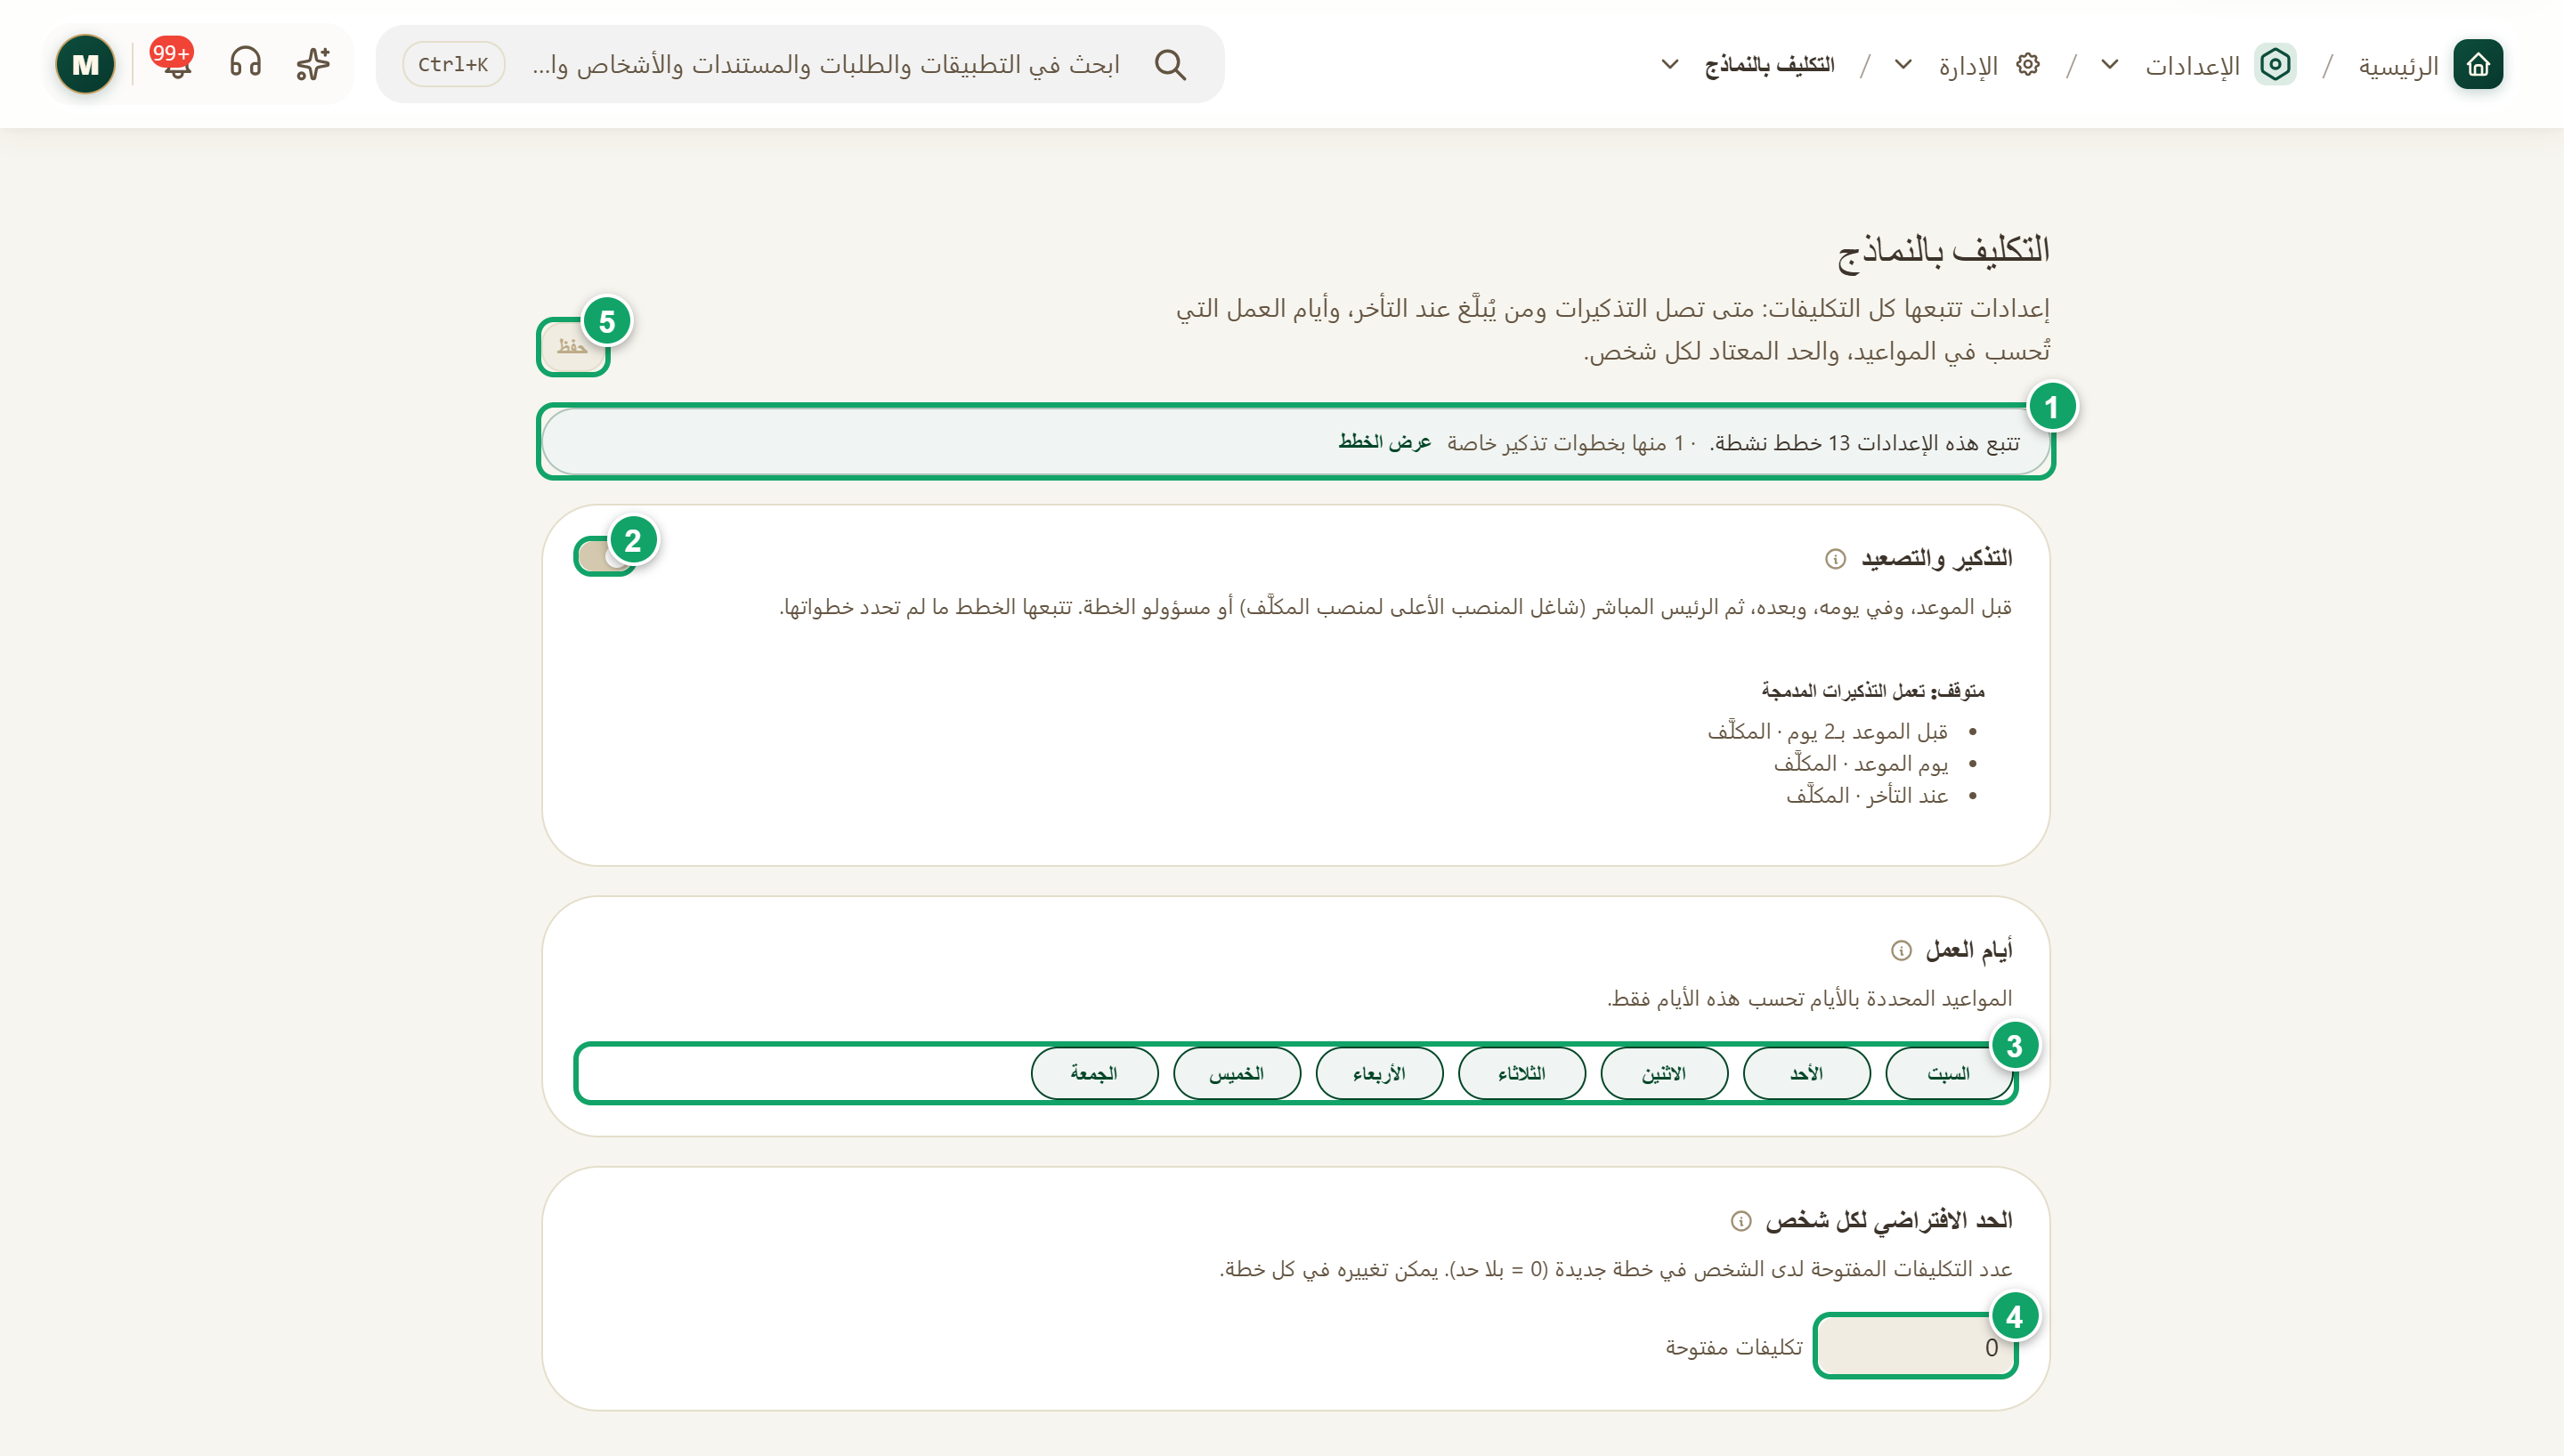
\includegraphics[width=0.95\linewidth,height=0.72\textheight,keepaspectratio]{figures/screens/ch08-form-assignments-ar.png}
\caption{صفحة التكليف بالنماذج}
\label{fig:settings-form-assignments-screen}
\shotnote{تعرض الصورة قيم مؤسسة الاختبار: التذكيرات المدمجة تعمل، وأيام الأسبوع السبعة كلها محتسبة، ولا حد للتكليفات. وهذه هي القيم الأصلية حتى تحفظ المؤسسة غيرها، فالمدة بالأيام تشمل عطلة نهاية الأسبوع إذا لم توقف أيامها. ① شريط يبين عدد الخطط النشطة التي تتبع هذه الإعدادات، ومعه رابط «عرض الخطط». ② مفتاح «التذكير والتصعيد». ③ «أيام العمل»: اضغط اليوم لإيقافه أو تشغيله، ويبقى يوم واحد على الأقل. ④ «الحد الافتراضي لكل شخص». ⑤ «حفظ».}
\end{figure}

\begin{figure}[H]
\centering
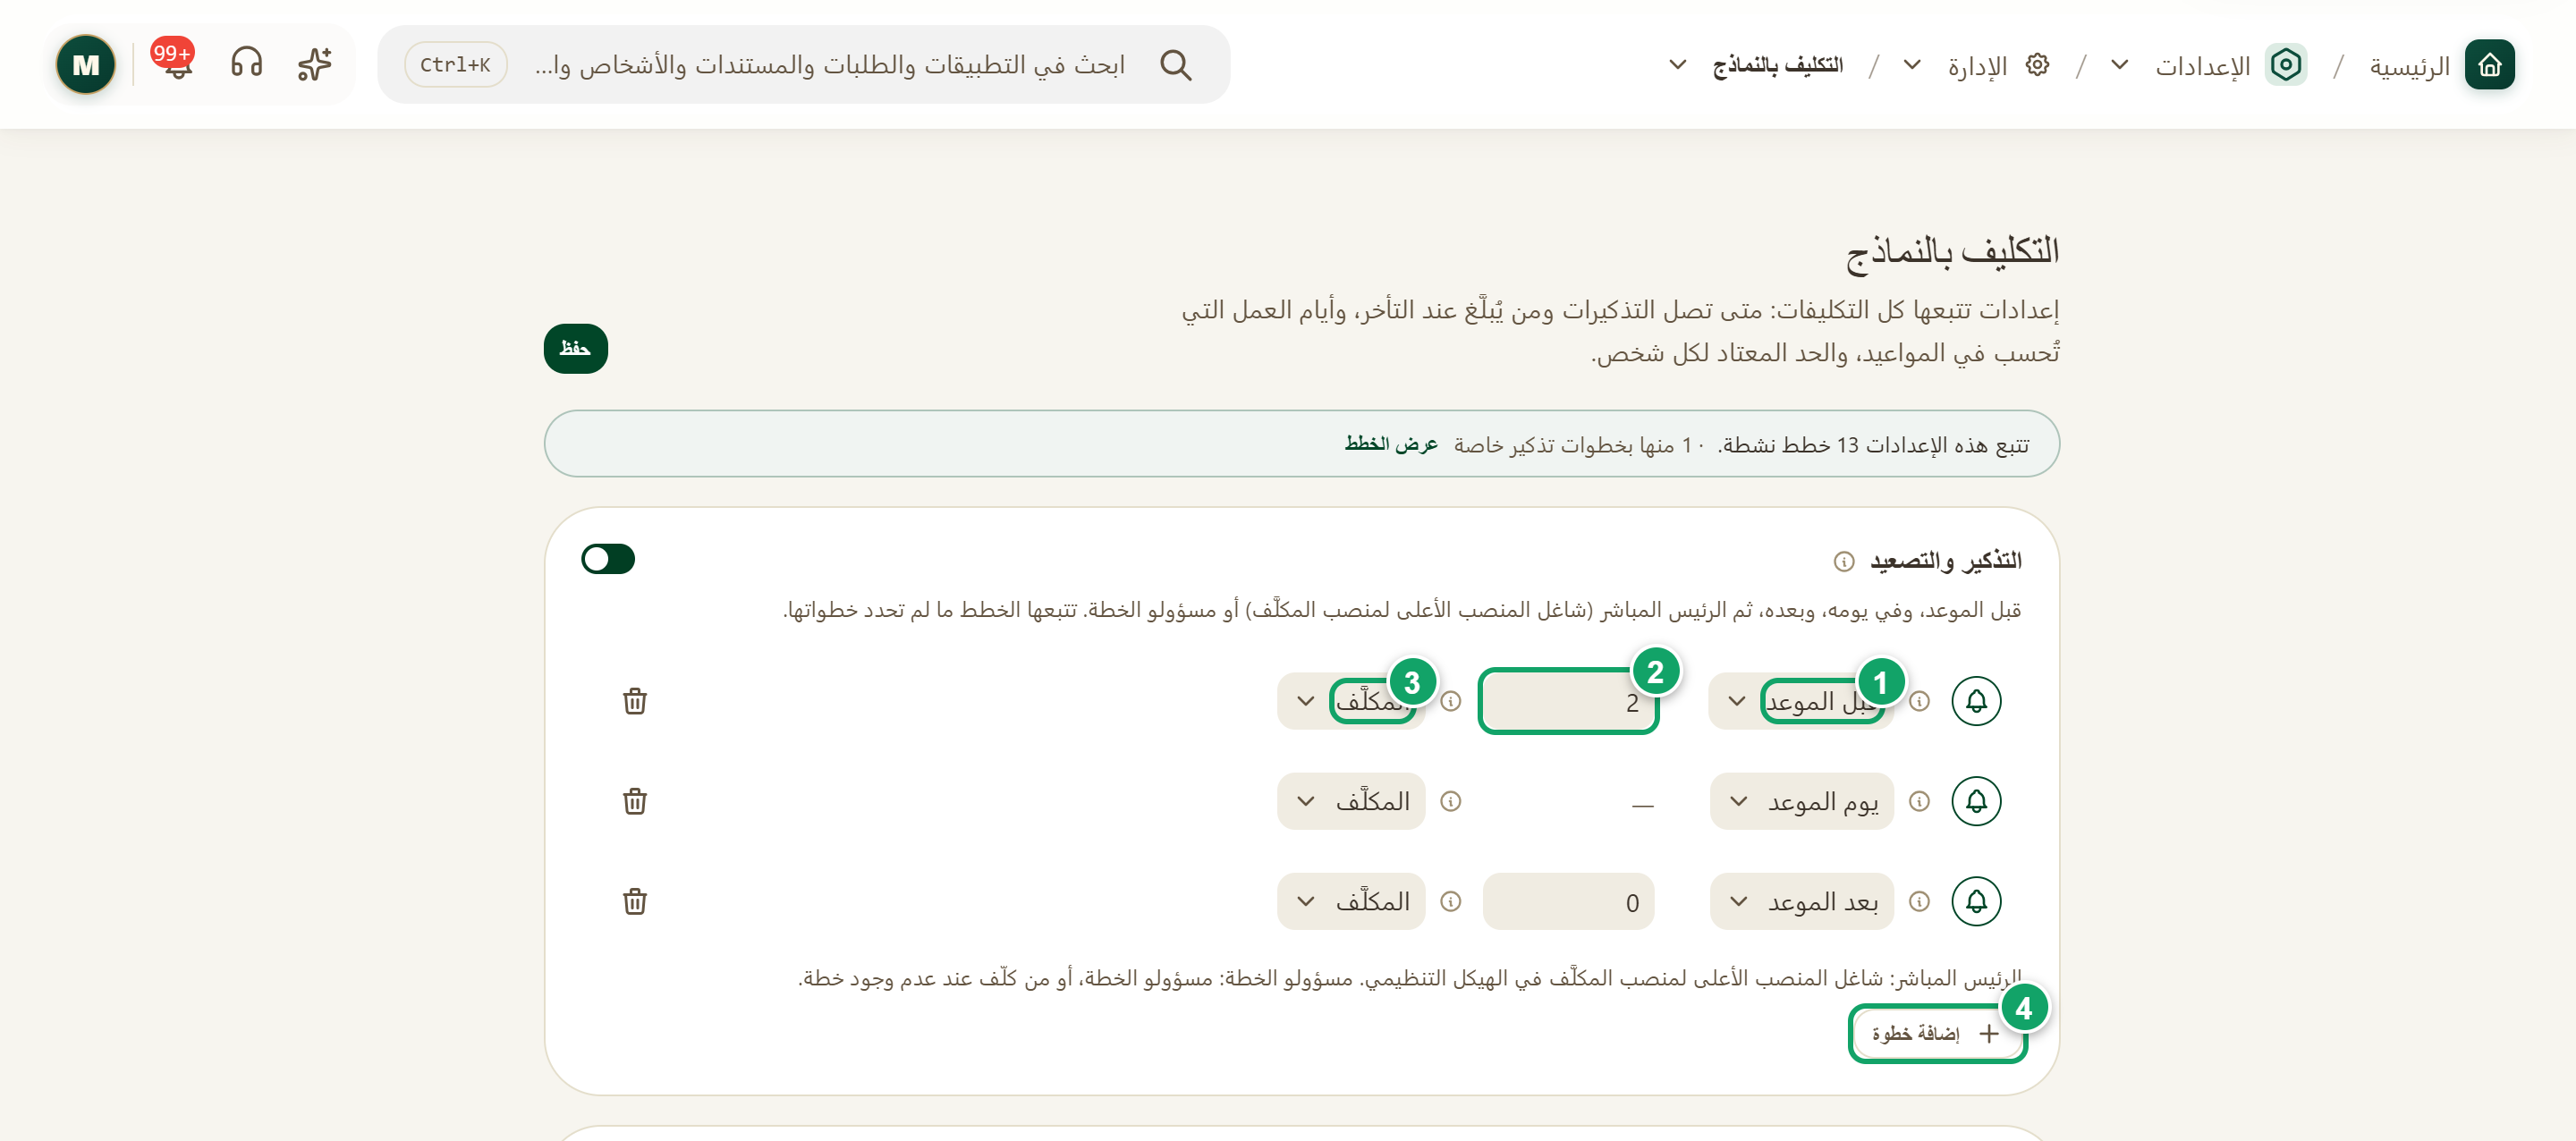
\includegraphics[width=0.95\linewidth,height=0.72\textheight,keepaspectratio]{figures/screens/ch08-form-assignments-ladder-ar.png}
\caption{خطوات التذكير عند تشغيل المفتاح}
\label{fig:settings-form-assignments-ladder-screen}
\shotnote{تعرض الصورة المفتاح مشغلاً دون حفظ، وتبدأ الخطوات بنسخة من التذكيرات المدمجة لتعدّل عليها بدل البدء من الصفر. كل صف خطوة تجيب عن سؤالين: متى يُرسل التذكير، ولمن. ① متى: «قبل الموعد» أو «يوم الموعد» أو «بعد الموعد». ② عدد الأيام، حتى 60 يوماً. ③ لمن: «المكلَّف» أو «رئيسه المباشر» أو «مسؤولو الخطة» أو «بالكود». ④ «إضافة خطوة»: حتى 8 خطوات.}
\end{figure}

\begin{table}[H]
\centering
\caption{ماذا تسجل في التكليف بالنماذج؟}
\label{tab:settings-form-assignments-fields}
\begin{tabularx}{\linewidth}{R{4.2cm} Y}
\rcHeaderRow
\thh{الإعداد} & \thh{ما الذي تسجله فيه؟}\\
«التذكير والتصعيد» & عند الإيقاف تعمل التذكيرات المدمجة للمكلَّف: قبل الموعد بيومين، ويوم الموعد، وعند التأخر. وعند التشغيل تعمل خطواتك. وتتبعها الخطط ما لم تحدد خطوات خاصة بها.\\
«رئيسه المباشر» & شاغل المنصب الأعلى لمنصب المكلَّف في الهيكل التنظيمي.\\
«مسؤولو الخطة» & المسؤولون عن الخطة، أو من أصدر التكليف إذا لم تكن هناك خطة.\\
«بالكود» & تعبير يحسب المستلمين، ويحتاج إلى من يعرف كتابة التعابير. استخدم الخيارات الثلاثة الأخرى إذا كانت تكفيك.\\
«أيام العمل» & الأيام التي تُحسب في المواعيد المحددة بالأيام.\\
«الحد الافتراضي لكل شخص» & عدد التكليفات المفتوحة لدى الشخص في خطة جديدة، من 0 إلى 500، و0 تعني بلا حد. ويمكن تغييره في كل خطة.\\
\end{tabularx}
\end{table}

\begin{enumerate}
\item من «الإعدادات» افتح «التكليف بالنماذج»، واقرأ الشريط لتعرف عدد الخطط المتأثرة.
\item شغّل «التذكير والتصعيد»، ثم عدّل الخطوات أو أضف خطوة بعد الموعد إلى «رئيسه المباشر».
\item حدّد «أيام العمل»، ثم اكتب «الحد الافتراضي لكل شخص».
\item اضغط «حفظ».
\end{enumerate}

\textbf{تحقق:} تظهر رسالة «تم الحفظ.» وتبقى القيم عند إعادة فتح الصفحة. وتبقى الخطة التي لها خطوات خاصة على خطواتها، ويبين الشريط عدد هذه الخطط. أما الحد الجديد فيبدأ من الخطط الجديدة.

\clearpage
\section{تصنيفات الفحوص}
\label{sec:settings-feature-check-categories}

الفحص قاعدة في النموذج تنبّه المراجع إلى قيمة تحتاج إلى نظر. وتحدد هذه الصفحة التصنيفات التي تُرتَّب تحتها الفحوص، مثل الاتساق أو الطاقة الاستيعابية، ليتمكن المراجعون ولوحات المعلومات من تجميعها بحسب التصنيف. تحتاج إليها عندما تكثر الفحوص ويصعب تتبعها. يقرأ أي عضو هذه التصنيفات، ويغيّرها مالك المؤسسة وحاملو دور المسؤول فقط.

\begin{rcnote}[مثال: شركة الأفق]
يضغط مسؤول النظام «إضافة تصنيف» عند ④، ويكتب «بيانات الفرع» عند ①، ويختار لونه عند ②، ثم يضغط «حفظ» عند ⑤. بعد ذلك تختار سارة الخطيب هذا التصنيف لفحص في نموذج طلب الزيارة.
\end{rcnote}

\begin{figure}[H]
\centering
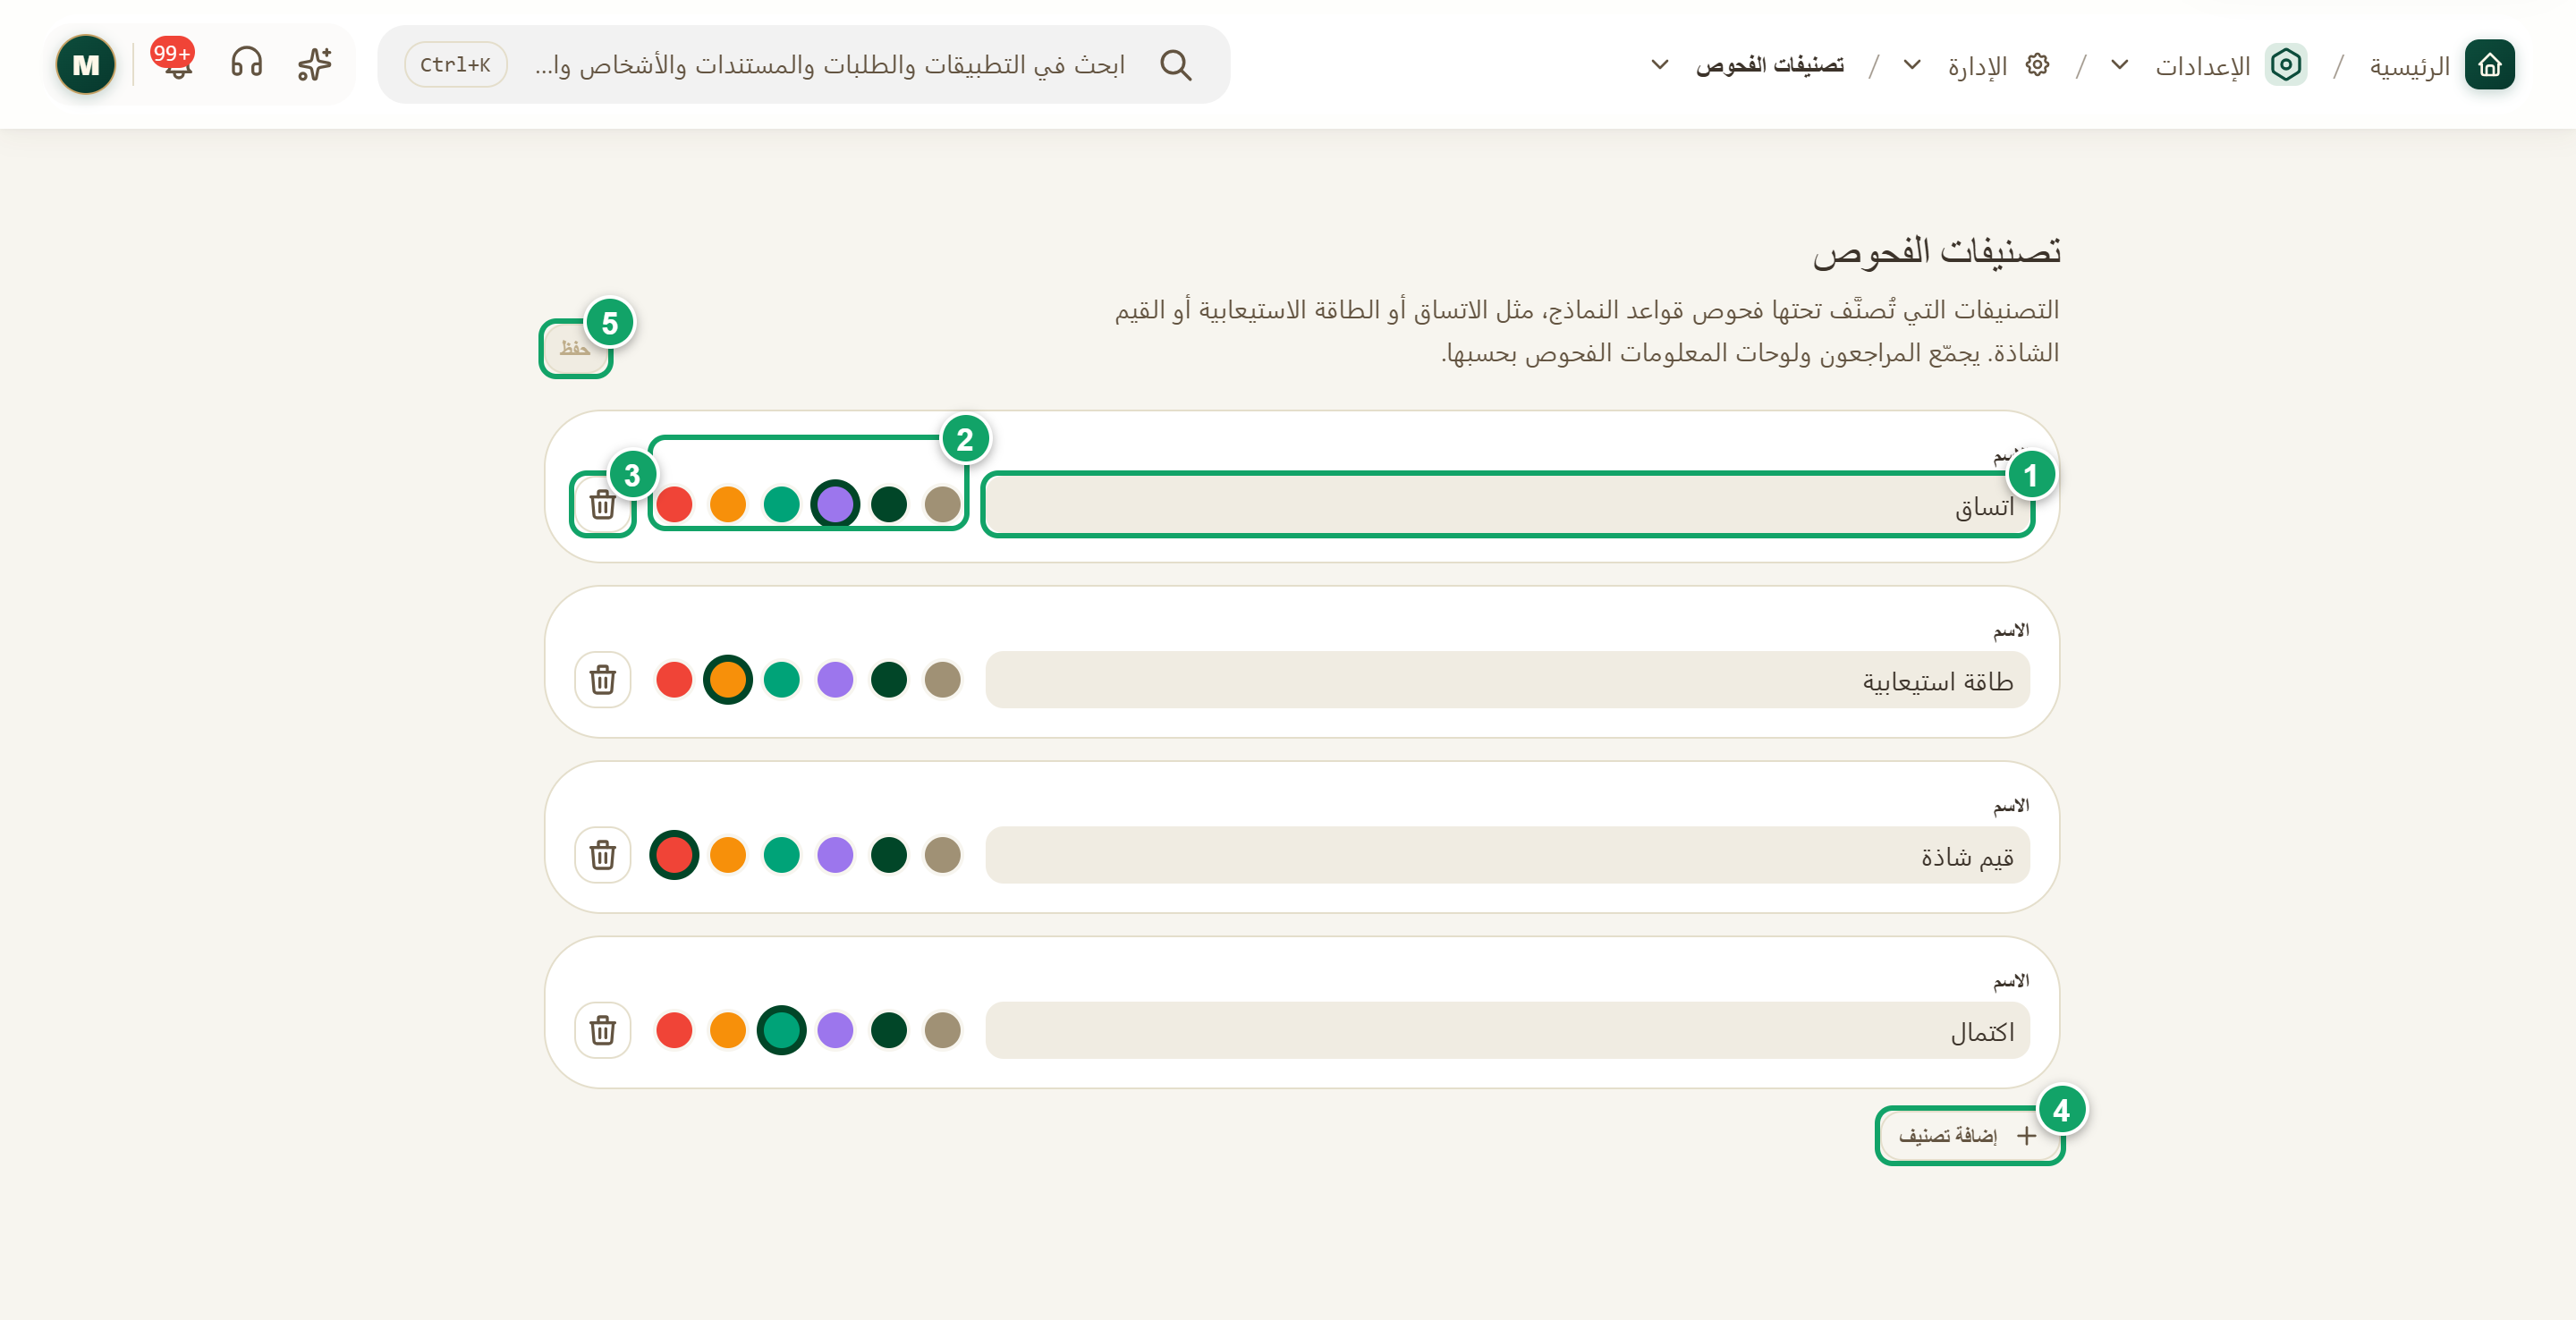
\includegraphics[width=0.95\linewidth,height=0.72\textheight,keepaspectratio]{figures/screens/ch08-check-categories-ar.png}
\caption{قائمة تصنيفات الفحوص}
\label{fig:settings-check-categories-screen}
\shotnote{تعرض الصورة التصنيفات الأربعة الموجودة في مؤسسة الاختبار، والتغيير هنا لا يسري حتى الضغط على «حفظ». فكل بطاقة تصنيف قابل للاختيار في قواعد النماذج، وإعادة تسميته تُبقي الفحوص المرتبطة به مجمَّعة تحته. ① «الاسم»: حتى 80 حرفاً، ويُكتب بكل لغة من أزرار اللغات. ② «اللون»: ستة ألوان. ③ «حذف التصنيف»: يختفي الصف دون رسالة تأكيد، ولا يكتمل الحذف إلا بالحفظ. ④ «إضافة تصنيف». ⑤ «حفظ»: يبقى معطلاً حتى يتغير شيء، ويتعطل إذا بقي تصنيف بلا اسم.}
\end{figure}

\begin{table}[H]
\centering
\caption{ماذا تسجل في تصنيف الفحص؟}
\label{tab:settings-check-categories-fields}
\begin{tabularx}{\linewidth}{R{4.2cm} Y}
\rcHeaderRow
\thh{الحقل} & \thh{ما الذي تسجله فيه؟}\\
«الاسم» & اسم التصنيف كما يراه المراجع، بلغة واحدة على الأقل. ويمكنك إضافة حتى 50 تصنيفاً.\\
«اللون» & لون يساعد على تمييز التصنيف، ويحصل التصنيف الجديد على لون أولي تستطيع تغييره.\\
\end{tabularx}
\end{table}

\begin{enumerate}
\item من «الإعدادات» افتح «تصنيفات الفحوص»، ثم اضغط «إضافة تصنيف».
\item اكتب «الاسم»، واختر «اللون».
\item اضغط «حفظ».
\item في قواعد النموذج، افتح الفحص واختر التصنيف من حقل «التصنيف».
\end{enumerate}

\textbf{تحقق:} تظهر رسالة «تم الحفظ.» ويبقى التصنيف في القائمة بعد إعادة فتح الصفحة. وإذا حذفت تصنيفاً تستخدمه قاعدة، فإن القاعدة تحتفظ به حتى تغيّره، ويظهر فيها بقيمته الداخلية، لذلك عدّل القواعد قبل الحذف.
